%-*- coding: UTF-8 -*-
% notes.tex
%
\documentclass[UTF8]{article}
\usepackage{geometry}
\geometry{a4paper, centering, scale=0.8}
\usepackage{minted}
\usepackage{hyperref}
\usepackage{indentfirst}    % to indent the first paragraph of a section
\usepackage{graphicx}       % to insert figures
\usepackage{amsmath}        % to type some math equations
\usepackage{amssymb}        % to use some special math font
\usepackage{IEEEtrantools}  % to use IEEEeqnarray
\usepackage{algorithm2e}    % to use algorithm environment
\usepackage{mathtools}      % to use \lfloor etc.
\usepackage{multicol}       % to display some content in multi-columns
\setlength{\columnseprule}{0.4pt}   % set the rule's width of multicols
\setlength{\columnsep}{5em}         % set the sep of multicols

% Math notation
% refered to https://github.com/exacity/deeplearningbook-chinese/blob/master/math_symbol.tex
\newcommand{\Scalar}[1]{\mathit{#1}}                % Scalar, the default math font
\newcommand{\Vector}[1]{\boldsymbol{\mathit{#1}}}   % Vector
\newcommand{\Matrix}[1]{\boldsymbol{\mathit{#1}}}   % Matrix
\newcommand{\Tensor}[1]{\textsf{\textbf{#1}}}       % Tensor
\newcommand{\Set}[1]{\mathbb{#1}}                   % Set
\newcommand{\Cal}[1]{\mathcal{#1}}                  % Math Cal

% Draw the lines in a matrix, which is composed by a series of vectors
\newcommand{\vRule}{\rule{0.3pt}{10mm}}             % vertical rule
\newcommand{\hRule}{\,\rule[1mm]{10mm}{0.3pt}\,}    % horizontal rule

% Ceil and floor
\DeclarePairedDelimiter\ceil{\lceil}{\rceil}
\DeclarePairedDelimiter\floor{\lfloor}{\rfloor}

\title{Deep Learning Specialization \\
        Convolutional Neural Networks}
\author{Du Ang \\ \texttt{du2ang233@gmail.com} }
\date{\today}

\begin{document}
\maketitle

\tableofcontents
\newpage

\section{Foundations of Convolutional Neural Networks}
\subsection{Convolutional Neural Networks}
\subsubsection{Computer Vision}
\paragraph{Computer Vision problems}
\begin{itemize}
    \item Image Classfiication
    \item Object Detection
    \item Neural Style Transfer
\end{itemize}

One of the challenges of Computer Vision problems is that the input can be really big. We want to
use large images to train our model, and if we use a fully-connected network, the huge input
features and so many parameters are not feasible to train.

\subsubsection{Edge Detection Example}
\paragraph{Vertical edge detection}
The convolution operation in programming languages:
\begin{itemize}
    \item Python: \mintinline{python}{conv_forward}
    \item TensorFlow: \mintinline{python}{tf.nn.conv2d}
\end{itemize}

\begin{figure}[htb]
    \centering
    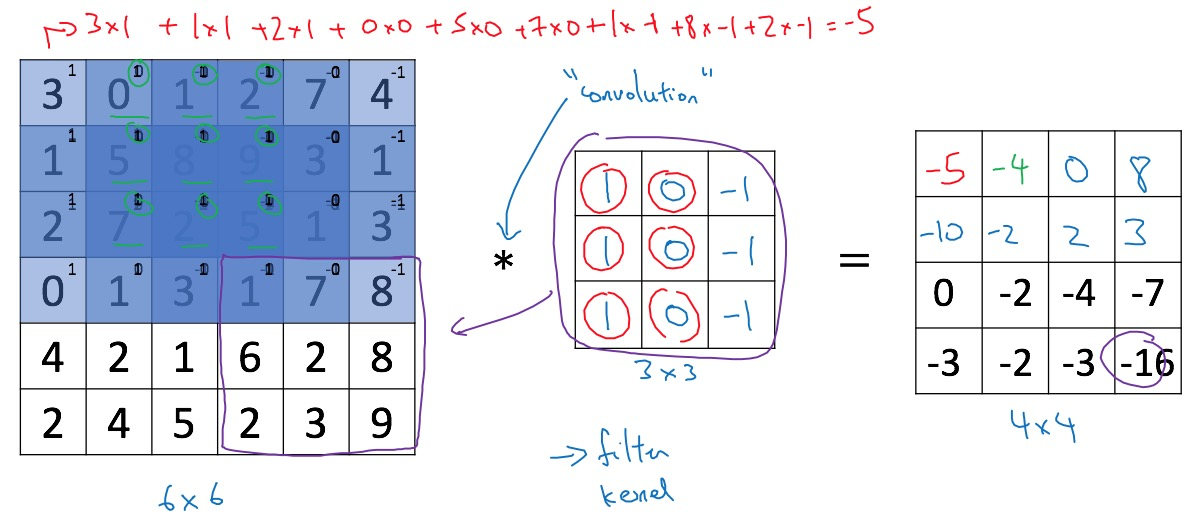
\includegraphics[width=40em]{figures/convolution-operation}
    \caption{The convolution operation for vertical edge detection}
    \label{fig:convolution-operation}
\end{figure}

\begin{figure}[htb]
    \centering
    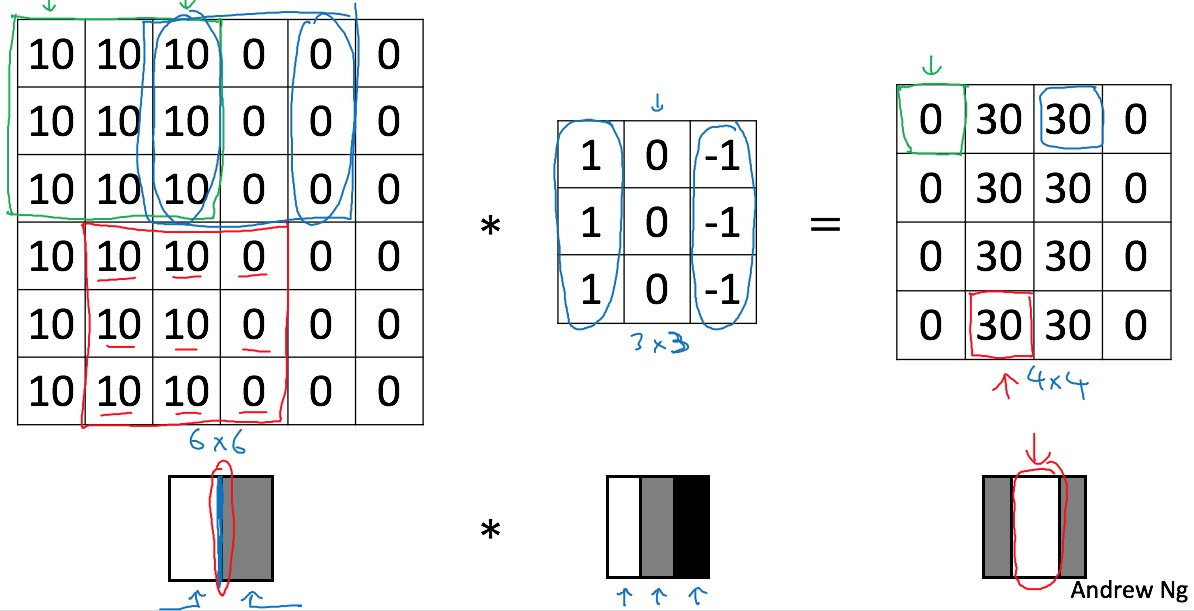
\includegraphics[width=40em]{figures/vertical-edge-detection-example}
    \caption{Vertical edge detection example for a simplified image}
    \label{fig:vertical-edge-detection-example}
\end{figure}

\subsubsection{More Edge Detection}
\begin{figure}[htb]
    \centering
    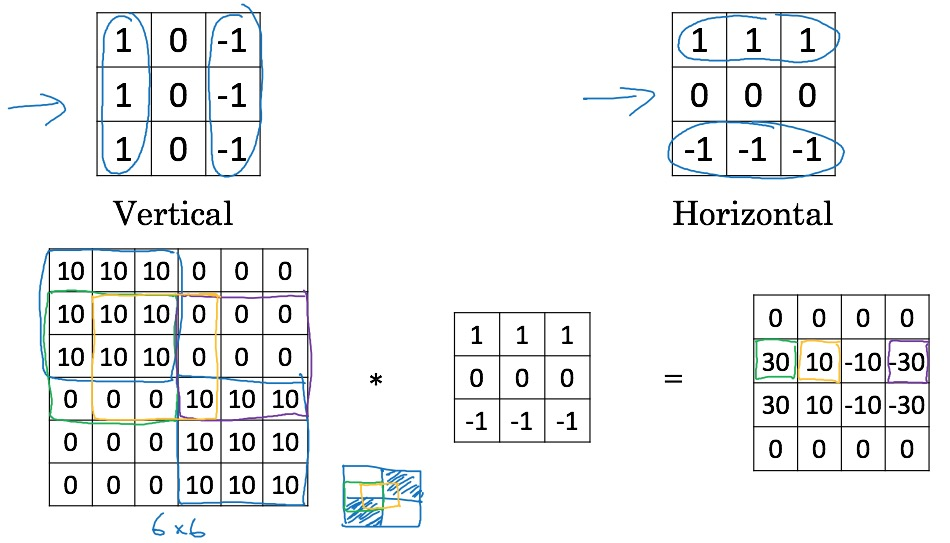
\includegraphics[width=40em]{figures/vertical-and-horizontal-edge-detection-example}
    \caption{Vertical and horizontal edge detection example}
    \label{fig:vertical-and-horizontal-edge-detection-example}
\end{figure}

\paragraph{Learning to detect edges}
Like Figure~\ref{fig:learning-to-detect-edges} shows, the idea that you can treat the nine numbers
in the filter as parameters, has been one of the most powerful ideas in computer vision.

\begin{figure}[htb]
    \centering
    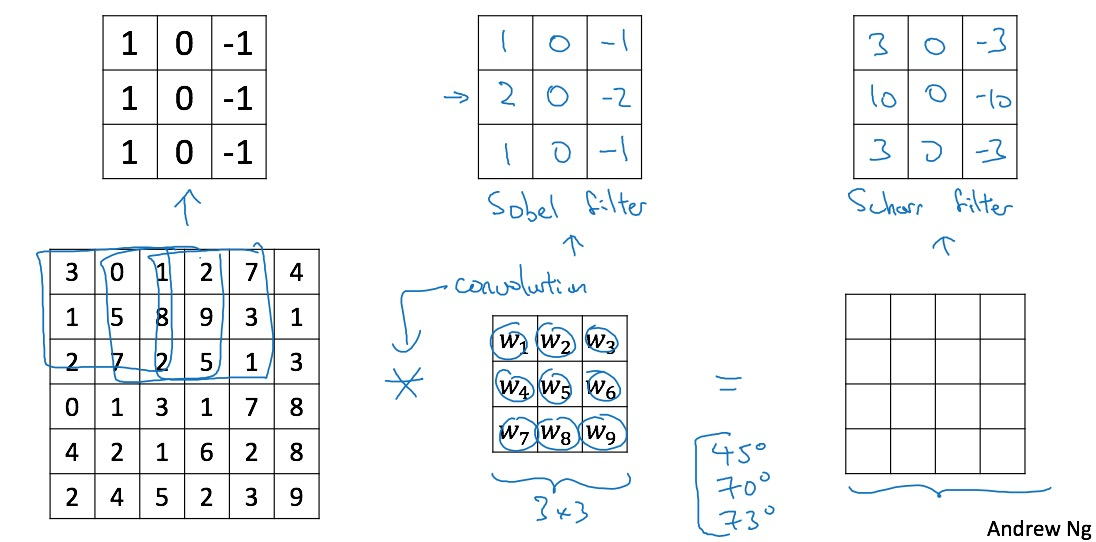
\includegraphics[width=40em]{figures/learning-to-detect-edges}
    \caption{Edge detection example with parameters to learn}
    \label{fig:learning-to-detect-edges}
\end{figure}

\subsubsection{Padding}
For a $n \times n$ image, use a $f \times f$ filter to do convolution, we will get a $(n-f+1) \times
(n-f+1)$ output.

The problems of no padding:
\begin{itemize}
    \item shrinking output
    \item throwing away information from edge
\end{itemize}

\paragraph{Valid and Same convolutions}
\begin{itemize}
    \item ``Valid'': $n \times n \* f \times f \rightarrow (n-f+1) \times (n-f+1)$
    \item ``Same'': Pad so that output size is the same as the input size.
    If we add padding $p$, the output will be $(n+2p-f+1) \times (n+2p-f+1)$, $\displaystyle
    p = \frac{f-1}{2}$. In convention, $f$ is usually odd.
\end{itemize}

\subsubsection{Strided Convolutions}
Strided convolutions is another piece of the basic builiding block of convolutions as used in
convolutional neural networks.

\begin{figure}[htb]
    \centering
    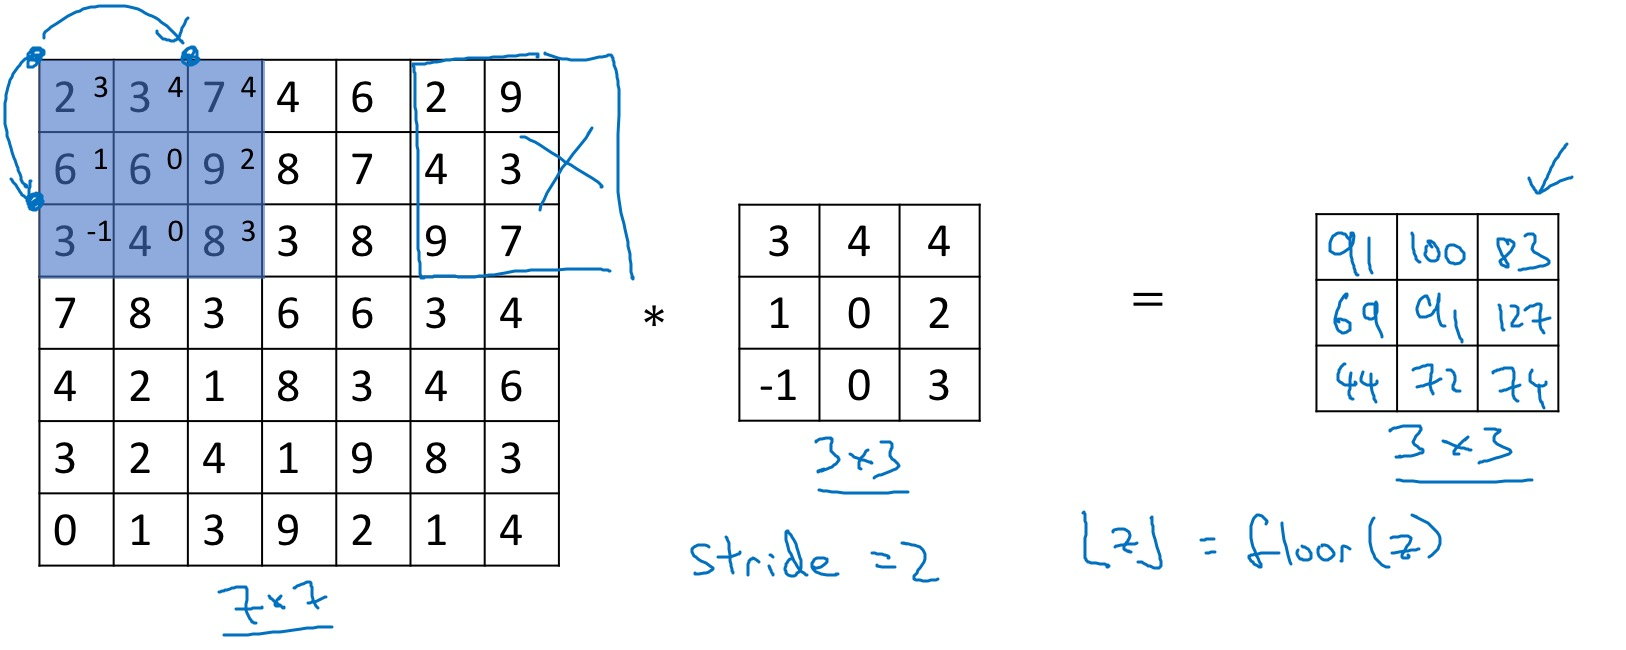
\includegraphics[width=40em]{figures/strided-convolution}
    \caption{Strided convolution example with stride 2}
    \label{fig:strided-convolution}
\end{figure}

$$ n \times n \text{ image (padding } p \text{)} \quad * \quad f \times f \text{ filter (stride }
s \text{)}  \quad \rightarrow \quad \floor*{\frac{n+2p-f}{s}+1} \times \floor*{\frac{n+2p-f}{s}+1}$$

\paragraph{Technical note on cross-correlation vs. convolution}
Convolution in math textbook and sigal processing has an extra mirroring operation, but in Deep
Learning, we've skipped it by convention. Technically, what we're actually doing, is sometimes
called cross-correlation instead of convolution.

The real convolution has the property called associativity in mathematics, which means $(A * B) * C
= A * (B * C)$. This is nice for some signal processing applications, but for deep neural networks,
it really doesn't matter.

\subsubsection{Convolutions Over Volume}
Figure~\ref{fig:convolutions-on-rgb-image} shows the example of convolutions over volume.

\begin{figure}[htb]
    \centering
    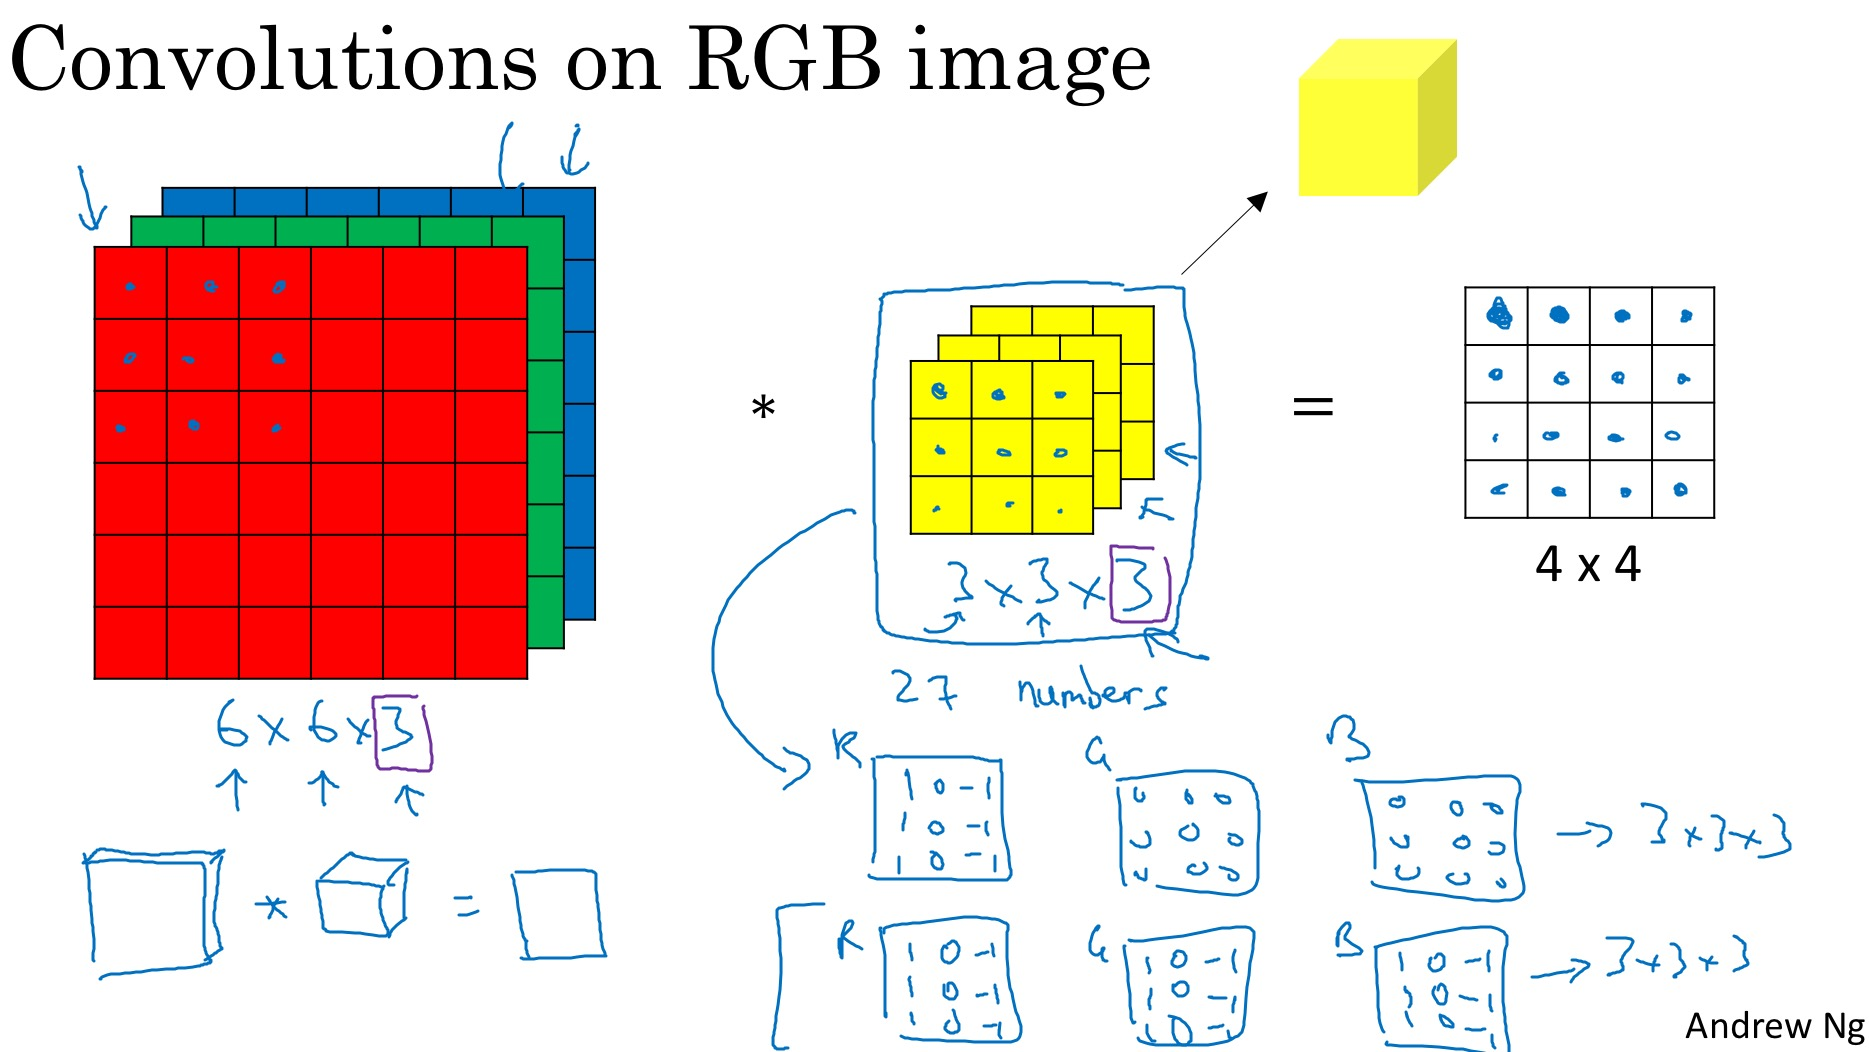
\includegraphics[width=40em]{figures/convolutions-on-rgb-image}
    \caption{Convolutions on RGB image}
    \label{fig:convolutions-on-rgb-image}
\end{figure}

If we want to detect different features at the same time, we can use multiple filters. The output
will then have a number of channels equal to the features you are detecting.

Sometimes, the term ``channel'' is also called ``depth''.

\paragraph{Summary}
$$ n \times n \times n_C \quad * \quad f \times f \times n_C \quad \rightarrow \quad
(n-f+1) \times (n-f+1) \times n_C' \qquad (stride = 1, \text{no padding})$$

\subsubsection{One Layer of a Convolutional Network}
Figure~\ref{fig:example-of-a-conv-layer} shows an example of a layer of a convolutional network.

\begin{figure}[htb]
    \centering
    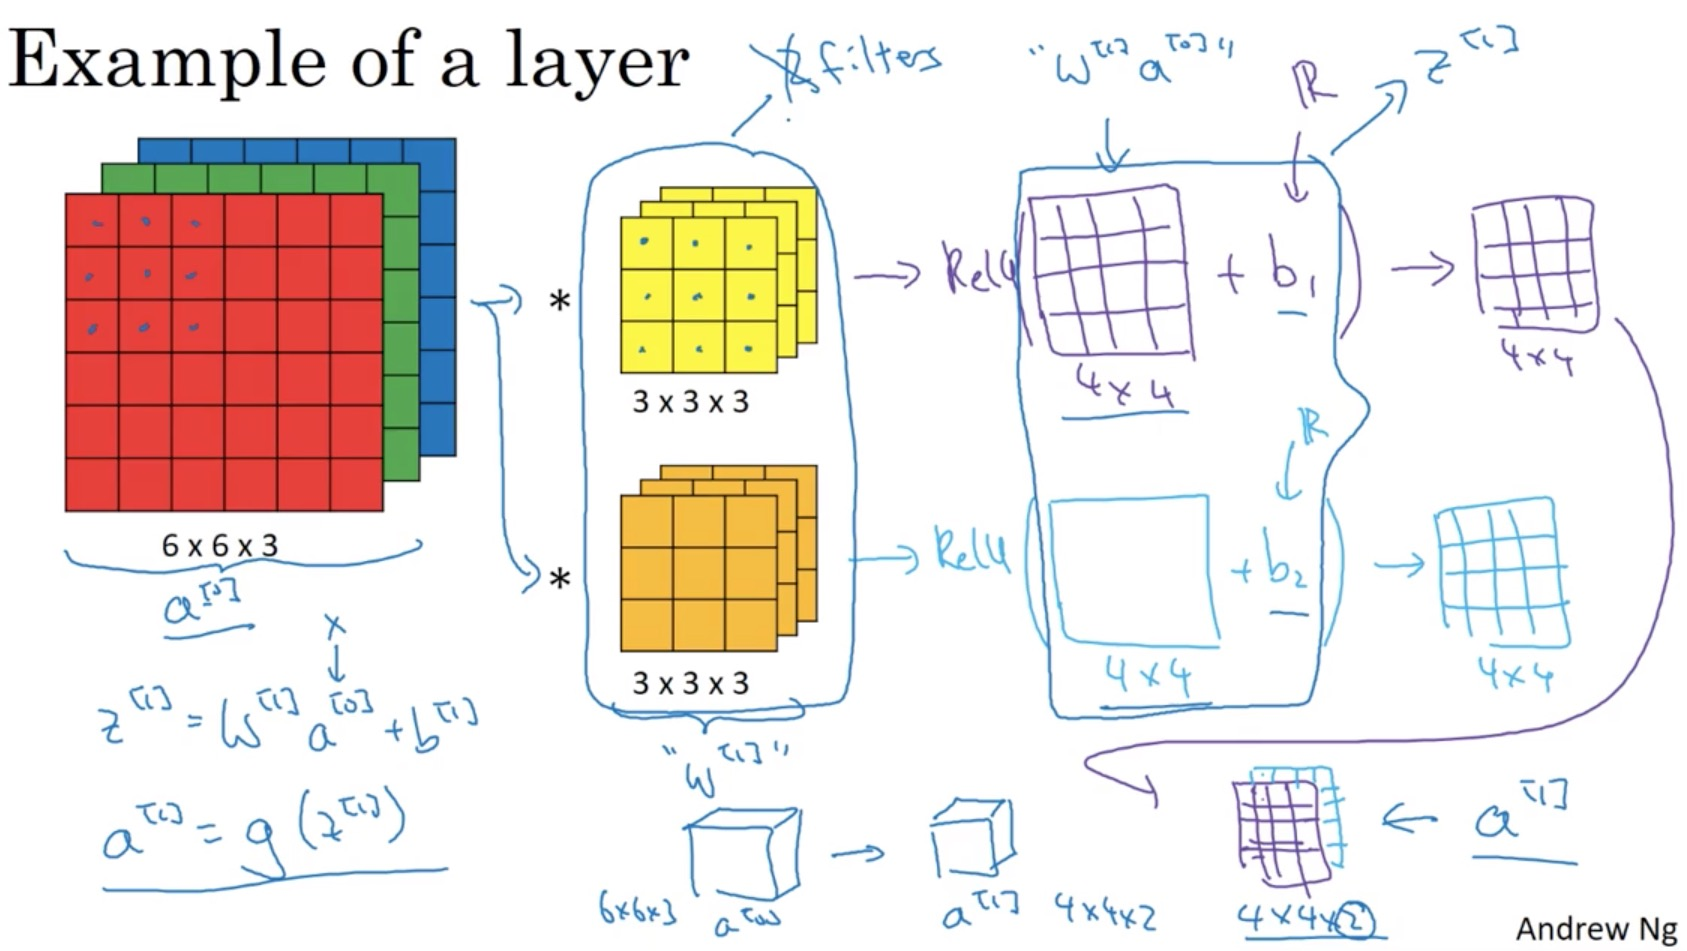
\includegraphics[width=40em]{figures/example-of-a-conv-layer}
    \caption{A example of a convolutional layer}
    \label{fig:example-of-a-conv-layer}
\end{figure}

\paragraph{Number of parameters in one layer}
If you have 10 filters that are $3 \times 3 \times$ in one layer of a neural network, how many
parameters does that layer have?
$$ (3 \times 3 \times 3 + 1) \times 10 = 280 $$

\paragraph{Summary of notation}
If layer $l$ is a convolution layer:
\begin{itemize}
    \item $f^{[l]} = \text{filter size}$
    \item $p^{[l]} = \text{padding}$
    \item $s^{[l]} = \text{stride}$
    \item $n_{\text{C}}^{[l]} = \text{number of filters}$
    \item Each filter is: $f^{[l]} \times f^{[l]} \times n_{\text{C}}^{[l]}$
    \item Activations: $\Vector{a}^{[l]} \rightarrow n_{\text{H}}^{[l]} \times n_{\text{W}}^{[l]} \times
    n_{\text{C}}^{[l]} \qquad \Matrix{A}^{[l]} \rightarrow m \times n_{\text{H}}^{[l]} \times
    n_{\text{W}}^{[l]} \times n_{\text{C}}^{[l]}$
    \item Weights: $f^{[l]} \times f^{[l]} \times n_{\text{C}}^{[l]} \times n_{\text{C}}^{[l-1]}$
    \item bias: $n_{\text{C}}^{[l]} \rightarrow (1, 1, 1, n_{\text{C}}^{[l]})$
    \item Input: $n_{\text{H}}^{[l-1]} \times n_{\text{W}}^{[l-1]} \times n_{\text{C}}^{[l-1]}$
    \item Output: $n_{\text{H}}^{[l]} \times n_{\text{W}}^{[l]} \times n_{\text{C}}^{[l]}$
    \item $\displaystyle n_{\text{H/W}}^{[l]} = \floor{\frac{n_{\text{H/W}}^{[l-1]} + 2p^{[l]}
    - f^{[l]}}{s^{[l]}} + 1}$
\end{itemize}

\subsubsection{Simple Convolutional Network Example}
A simple convolutional network example can be seen in Figure~\ref{fig:example-of-a-conv-layer}.

As you go deeper in the neural network, typically you start up with larger images, the height
and width will stay the same for a while, and gradually trend down as you go deeper in your
networks, whereas the number of channels will generally increase.

\begin{figure}[htb]
    \centering
    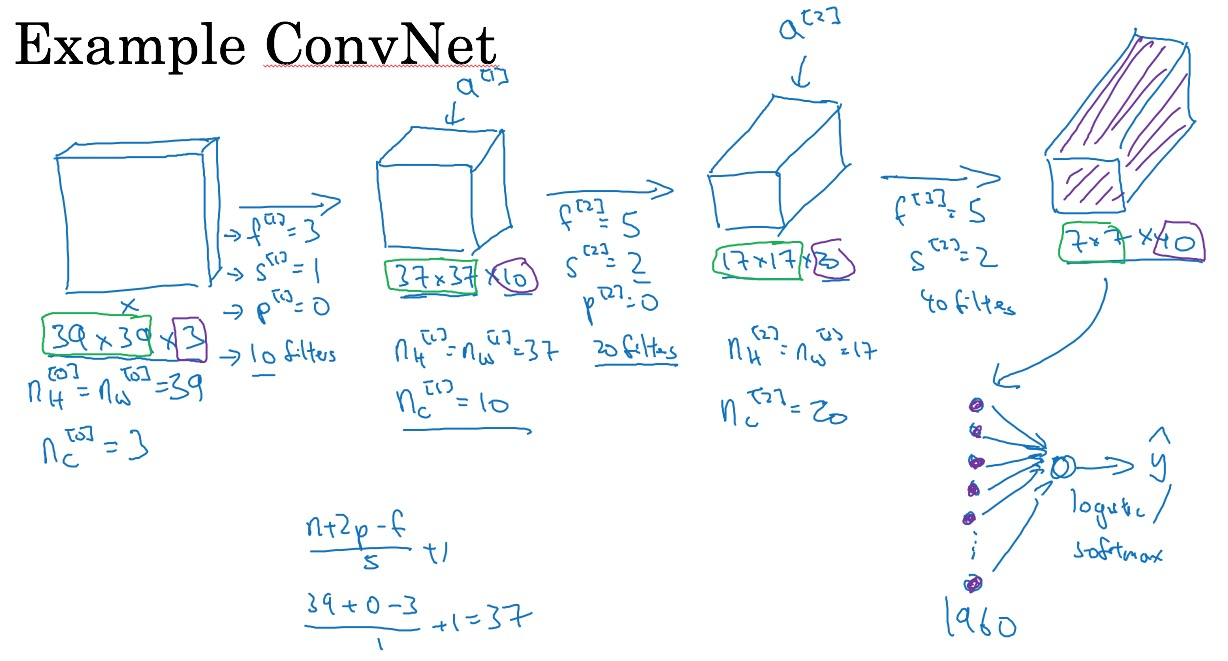
\includegraphics[width=40em]{figures/example-of-a-conv-net}
    \caption{A example of a convolutional network}
    \label{fig:example-of-a-conv-layer}
\end{figure}

Types of layers in a convolutional network:
\begin{itemize}
    \item Convolution (CONV)
    \item Pooling (POOL)
    \item Fully connected (FC)
\end{itemize}

\subsubsection{Pooling Layers}
Figure~\ref{fig:max-pooling} shows what max pooling is. As you can see, each coloured moving window
captures the maximum value within the widow is the output.

\begin{figure}[htb]
    \centering
    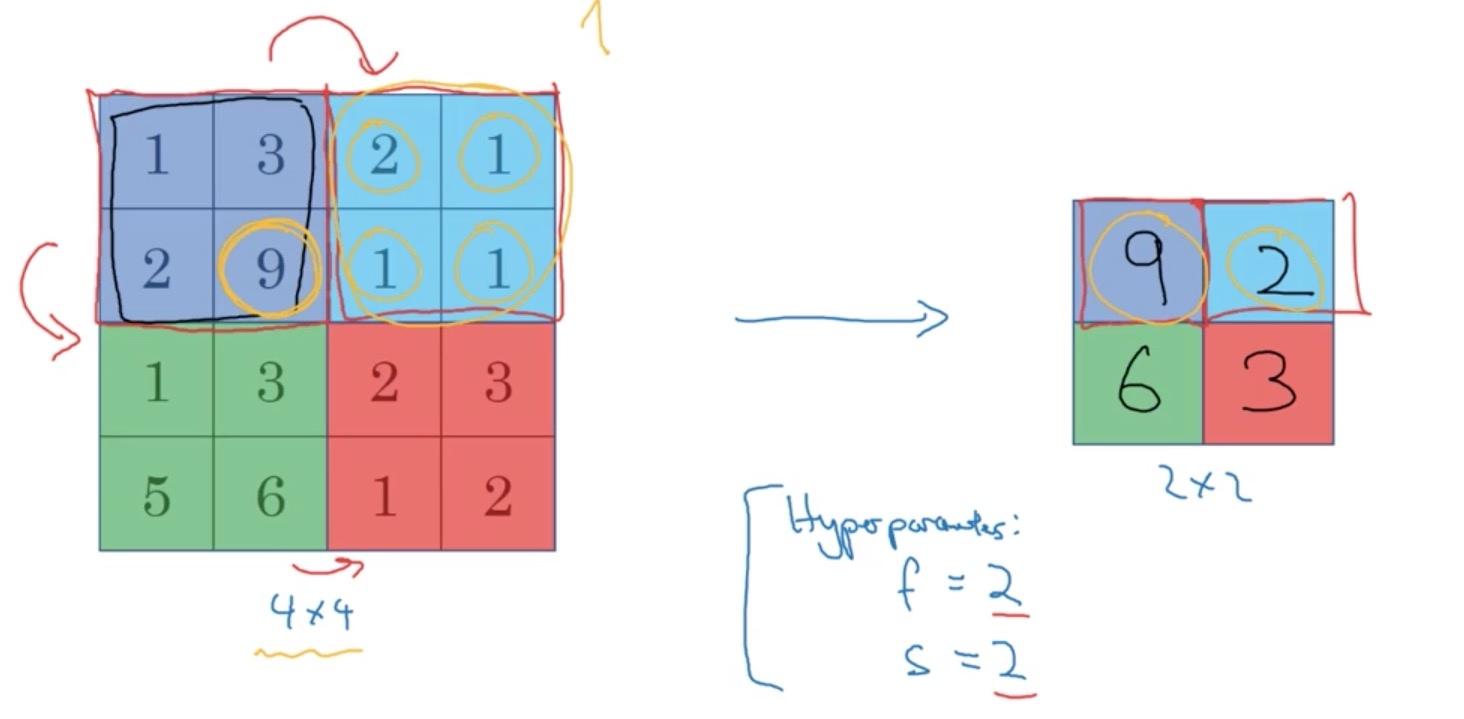
\includegraphics[width=40em]{figures/max-pooling}
    \caption{Max pooling}
    \label{fig:max-pooling}
\end{figure}

Figure~\ref{fig:average-pooling} shows a average pooling example. Instead of taking the maxes
within each filter, you take the average.

\begin{figure}[htb]
    \centering
    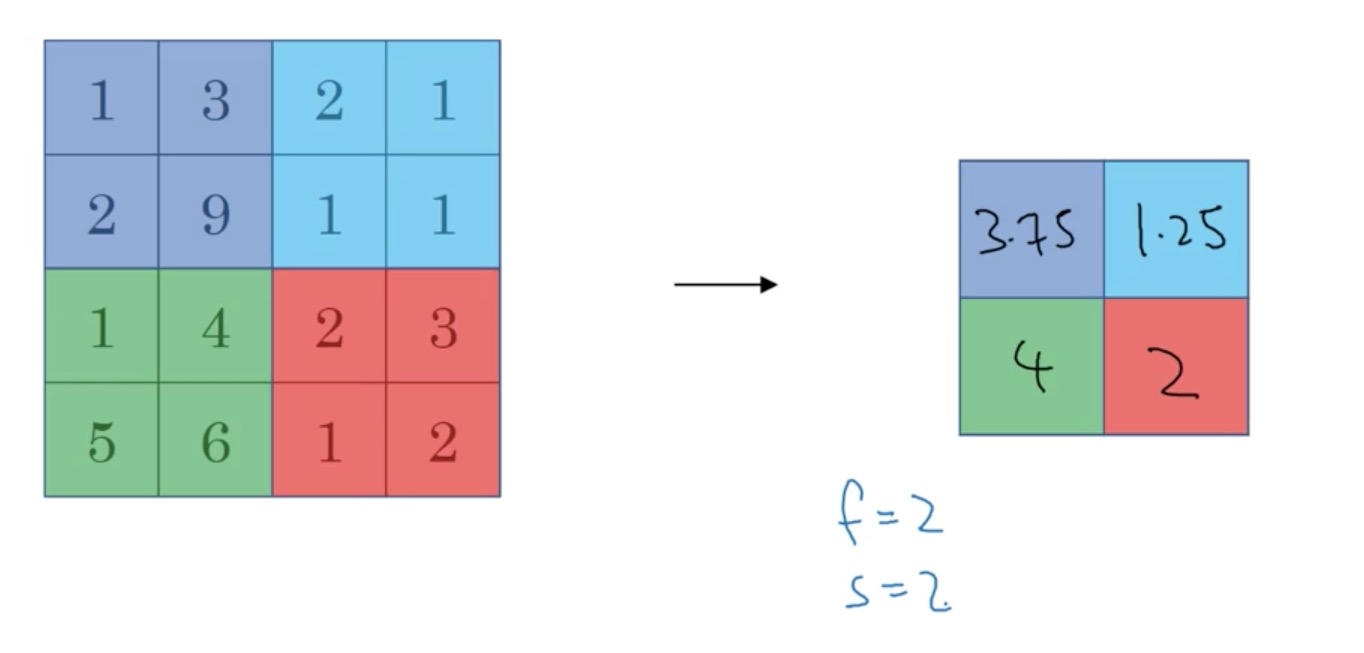
\includegraphics[width=40em]{figures/average-pooling}
    \caption{Average pooling}
    \label{fig:average-pooling}
\end{figure}

These days max pooling is used much more often than average pooling. With one exception, which is
sometimes, very deep in a neural network, you might use average pooling to collapse your
implementation from, say, $7 \times 7 \times 1000$, and average over all to get $1 \times 1 \times
1000$.

Hyperparameters (max or average pooling):
\begin{itemize}
    \item $f$: \text{filter size}
    \item $s$: \text{stride}
    \item ($p$: \text{padding}, little used)
\end{itemize}

Input: $ n_{\text{H}} \times n_{\text{W}} \times n_{\text{C}} $

Output: $\displaystyle \floor*{\frac{n_{\text{H}}-f}{s}+1} \times
\floor*{\frac{n_{\text{W}}-f}{s}+1} \times n_{\text{C}} $

Pooling layers have no parameters to learn.

\subsubsection{CNN Example}
Figure~\ref{fig:cnn-example} shows a CNN example inpired by LeNet-5.

In the literature of a Conv net, there are two conventions which are slightly in consistence about
what you call a layer. One convention is call CONV+POOL a layer. Another convention would be to
count the CONV layer as a layer, and the POOL layer as a layer. When people report a number of
layers in a neural network, usually people report just the number of layers that have weights
(parameters). In this class, we will use the first convention.

\begin{figure}[htb]
    \centering
    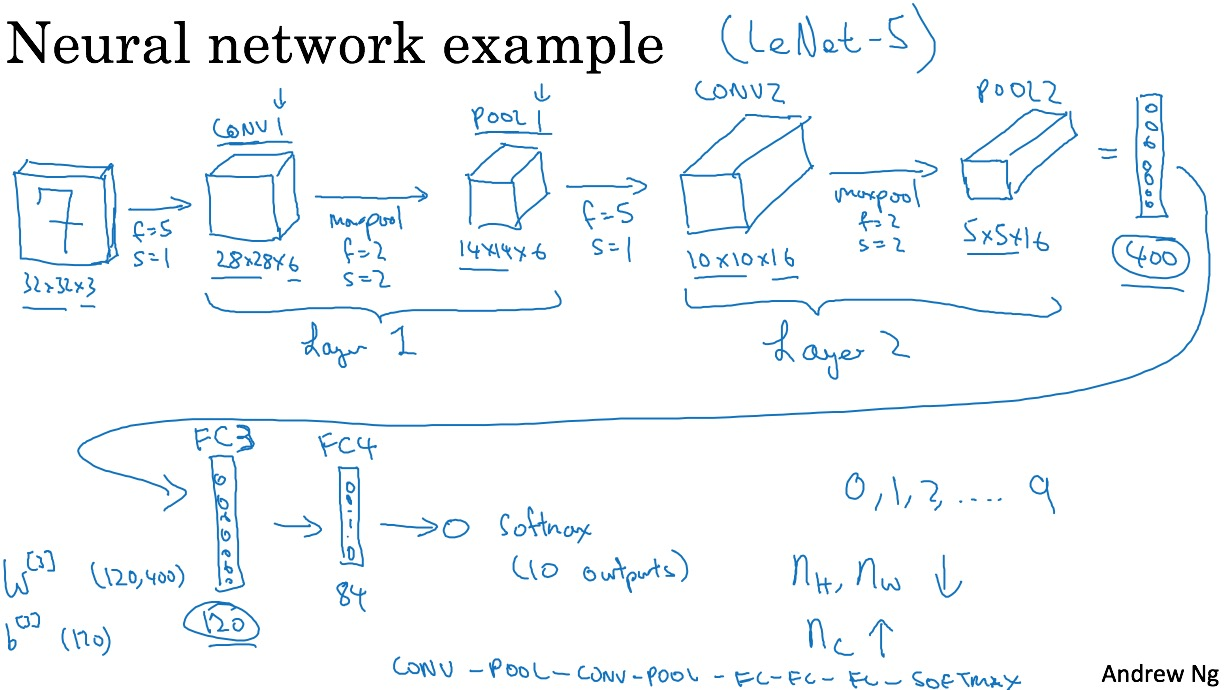
\includegraphics[width=40em]{figures/cnn-example}
    \caption{A CNN example, inspired by LeNet-5}
    \label{fig:cnn-example}
\end{figure}

\begin{figure}[htb]
    \centering
    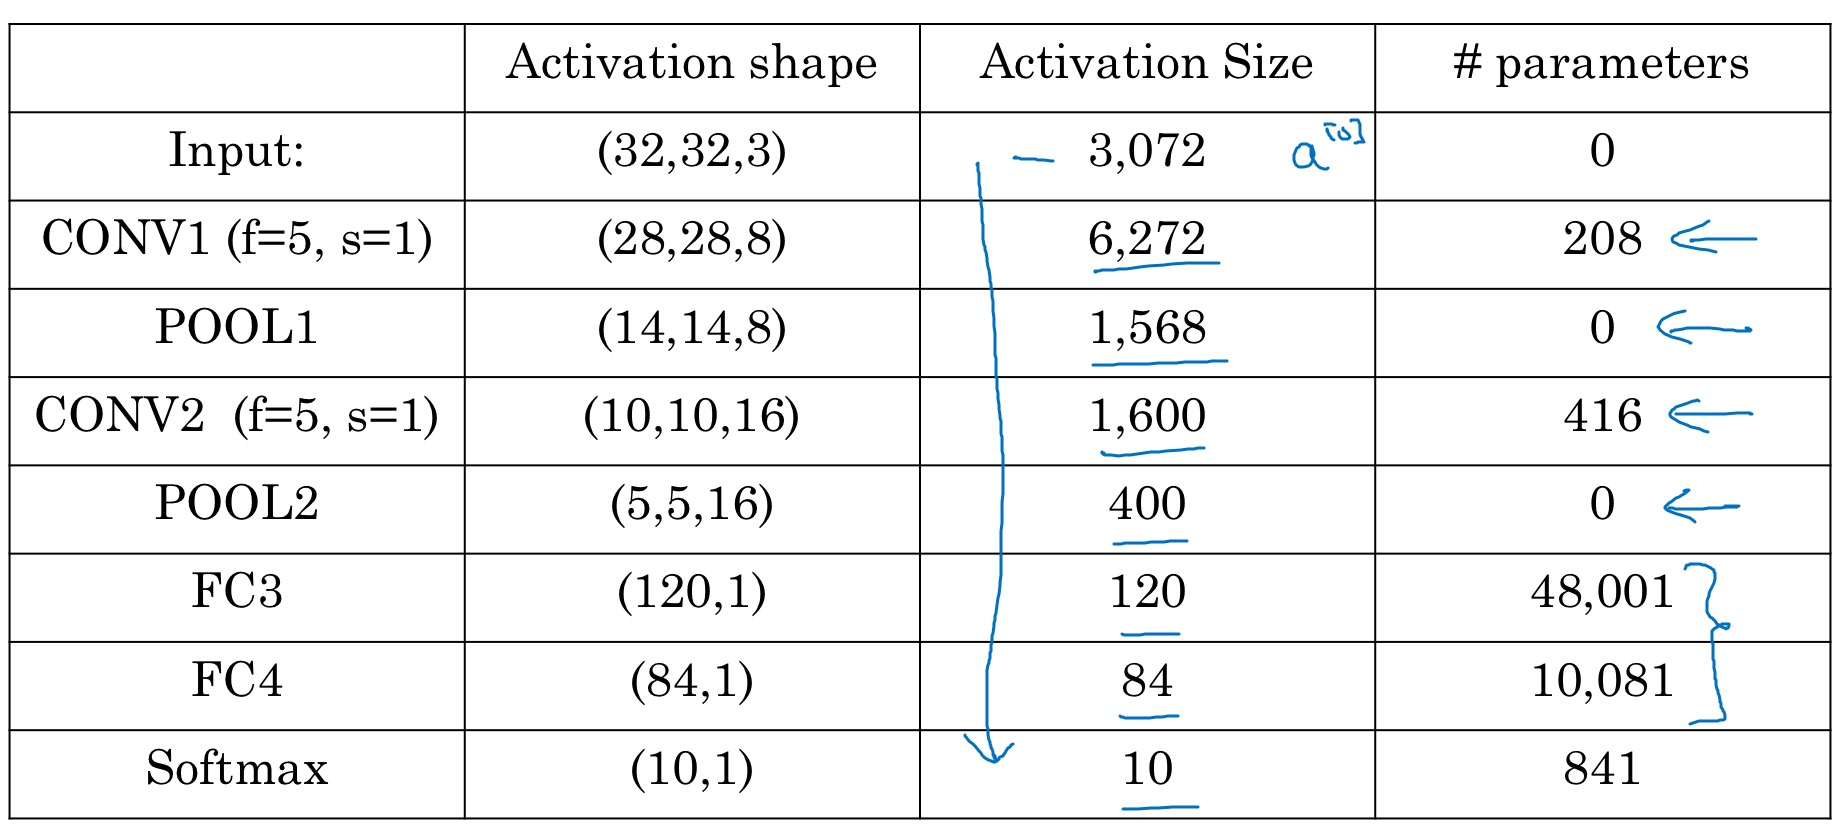
\includegraphics[width=40em]{figures/cnn-example-details}
    \caption{The details of a CNN example, inspired by LeNet-5}
    \label{fig:cnn-example-details}
\end{figure}

\subsubsection{Why Convolutions?}
There are two advantages of convolutional layers over just using fully-connected layers:
\begin{enumerate}
    \item Parameter sharing: A feature detector (such as a vertical edge detector) that's useful in
    one part of the image is probably useful in another part of the image.
    \item Sparsity of connections: In each layer, each output value depends only on a small number
    of inputs.
\end{enumerate}

Convolutional neural networks are very good at capturing translation of the areas, that's because
a convolutional structure helps the neural network encode the fact that an image shifted a few
pixels should result in pretty similar features and should probably be assigned the same output
label.

\section{Deep convolutional models: case studies}
\subsection{Case studies}
\subsubsection{Why look at case studies?}
One of the best ways for you to gain intuition yourself, is to read or to see other examples of
effective components. And it turns out that a neural network architecture that works well on one
computer vision task often works well on other tasks as well.

\paragraph{Outline}
\begin{itemize}
    \item Classic networks
    \begin{itemize}
        \item LeNet-5
        \item AlexNet
        \item VGG
    \end{itemize}
    \item ResNet
    \item Inception
\end{itemize}

\subsubsection{Classic Networks}
LeNet-5 (Figure~\ref{fig:lenet-5}), AlexNet (Figure~\ref{fig:alexnet}), VGG-16
(Figure~\ref{fig:vgg-16})

\begin{figure}[htb]
    \centering
    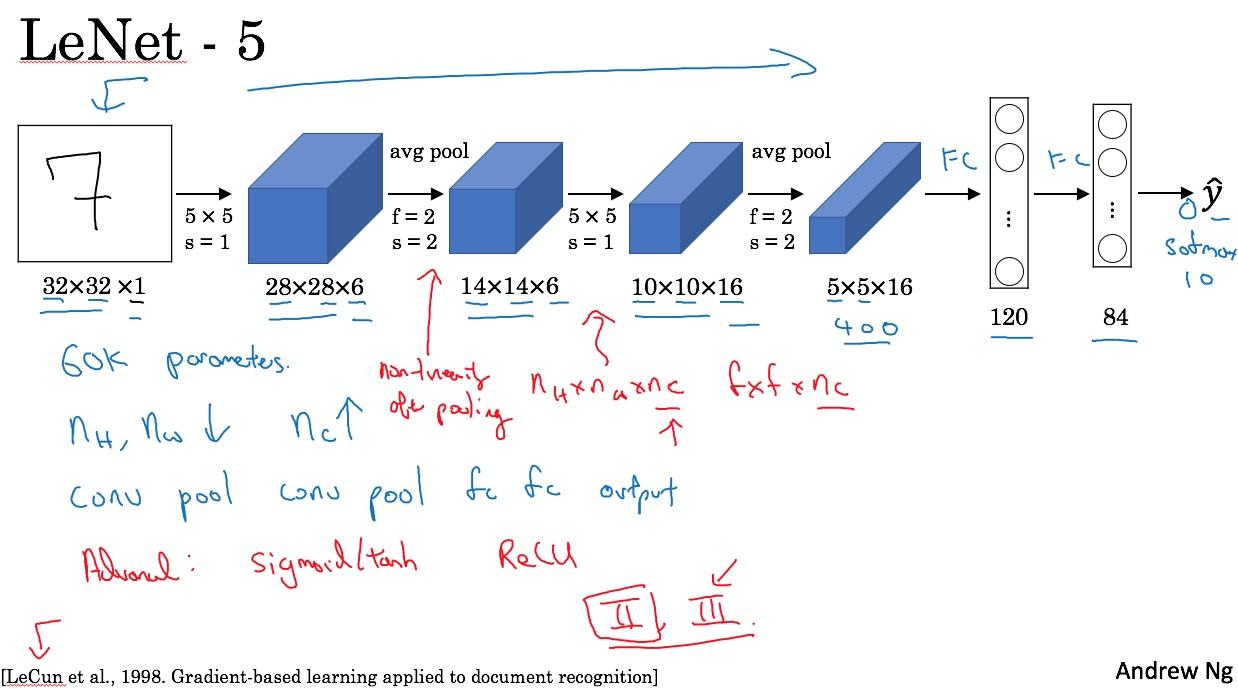
\includegraphics[width=40em]{figures/lenet-5}
    \caption{LeNet-5}
    \label{fig:lenet-5}
\end{figure}

\begin{figure}[htb]
    \centering
    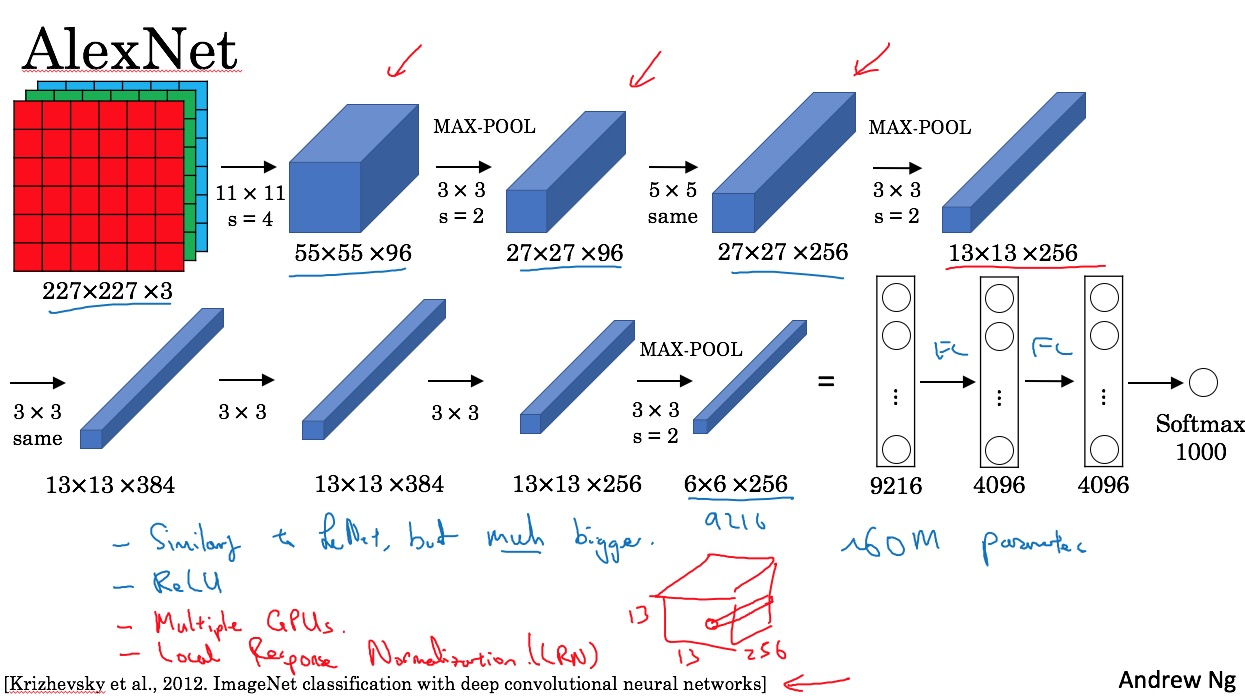
\includegraphics[width=40em]{figures/alexnet}
    \caption{AlexNet}
    \label{fig:alexnet}
\end{figure}

\begin{figure}[htb]
    \centering
    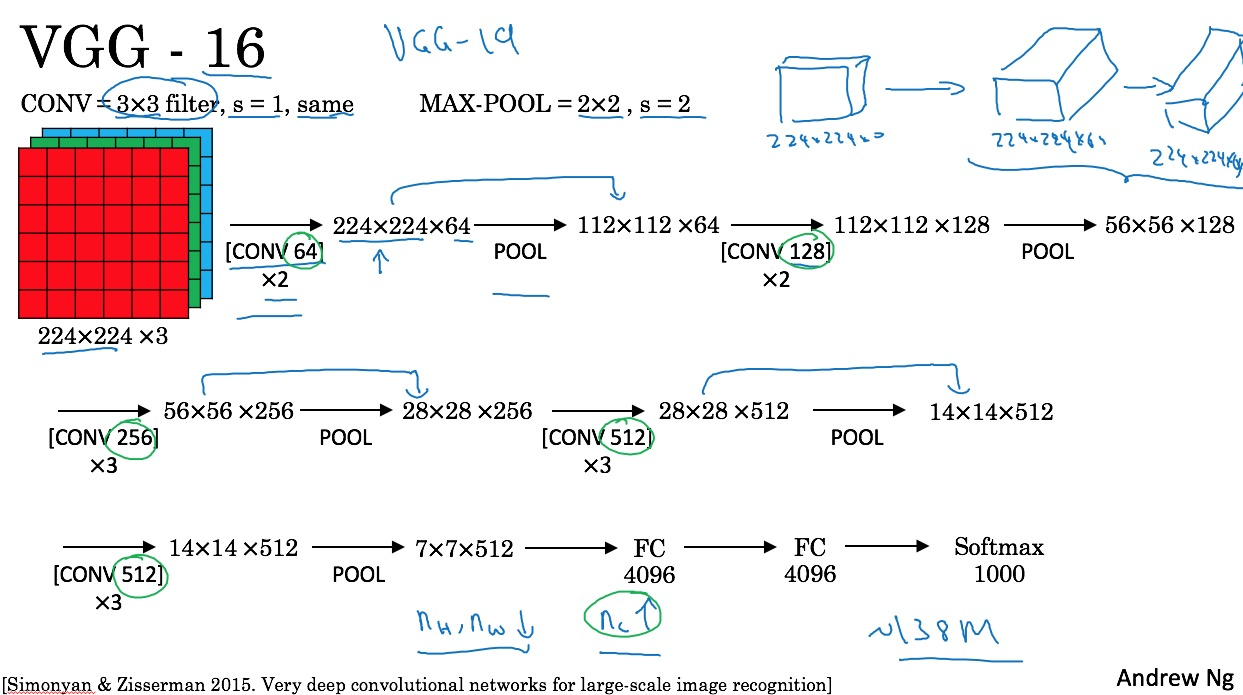
\includegraphics[width=40em]{figures/vgg-16}
    \caption{VGG-16}
    \label{fig:vgg-16}
\end{figure}

\subsubsection{ResNets}
Very, very deep neural networks are difficult to train because of vanishing and exploding gradients
types of problems. Skip connections of ResNets (Figure~\ref{fig:residual-block}) will allow you to
take the activation from one layer and suddenly feed it to another layer, even much deeper in the
neural network.

\begin{figure}[htb]
    \centering
    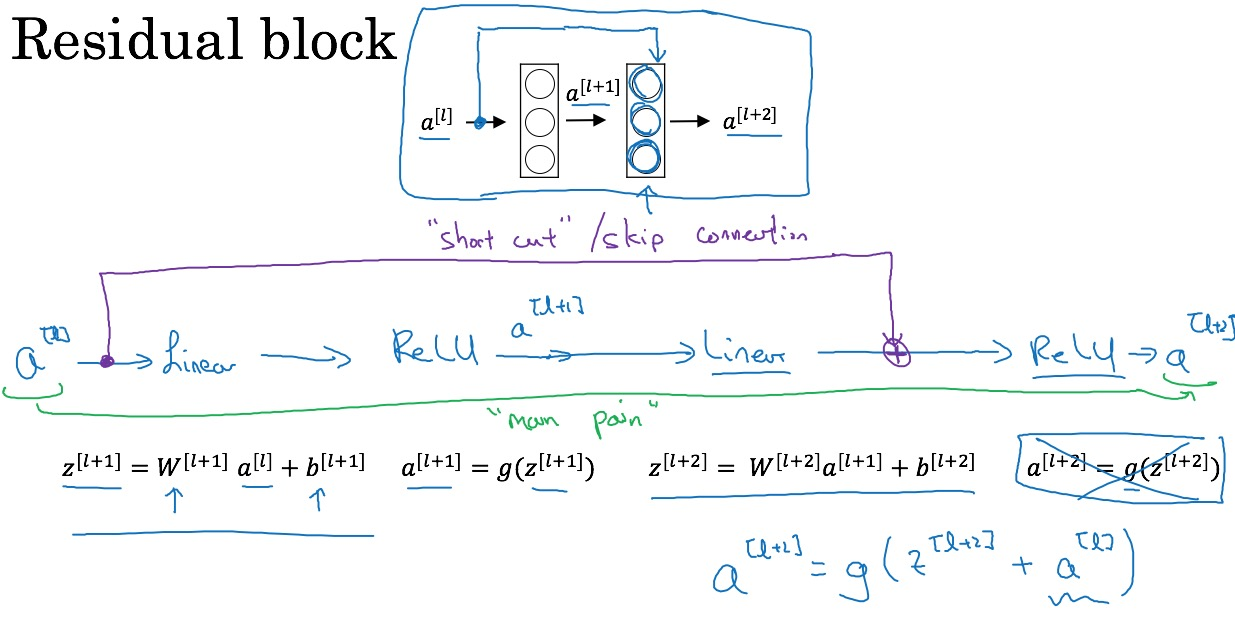
\includegraphics[width=40em]{figures/residual-block}
    \caption{Residual block}
    \label{fig:residual-block}
\end{figure}

$$ \Vector{z}^{[l+1]} = \Matrix{W}^{[l+1]} \Vector{a}^{[l]} + b^{[l+1]} $$
$$ \Vector{a}^{[l+1]} = g(\Vector{z^{[l+1]}}) $$
$$ \Vector{z}^{[l+2]} = \Matrix{W}^{[l+2]} \Vector{a}^{[l+1]} + b^{[l+2]} $$
$$ \Vector{a}^{[l+2]} = g(\Vector{z^{[l+2]}} + \Vector{a}^{[l]}) $$

To turn a ``plain network'' into ResNet, what you do is adding all those skip connections or
shortcut connections.

In theory, as you make a neural network deeper, it should only do better and better on the training
set. But in practice, or in reality, having a plain network that's very deep means that your
optimization algorithm just has a much harder time training, so your training error gets worse if
you pick a network that's too deep. But what happens with ResNets is that even as the number of
layers gets deeper, you can have the performance of the training error kind of keep on going down,
which can be seen in Figure~\ref{fig:plain-res-training-error-compare}.

\begin{figure}[htb]
    \centering
    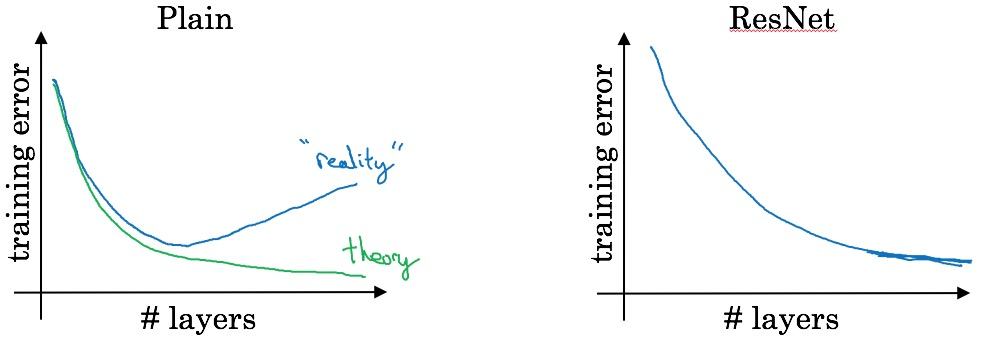
\includegraphics[width=40em]{figures/plain-res-training-error-compare}
    \caption{Comparing of the training error changes between Plain network and ResNet.}
    \label{fig:plain-res-training-error-compare}
\end{figure}

\subsubsection{Why ResNets Work}
$$ \Vector{a}^{[l+2]} = g(\Vector{z^{[l+2]}} + \Vector{a}^{[l]}) $$
$\Vector{z}^{[l+2]} = \Matrix{W}^{[l+2]} \Vector{a}^{[l+1]} + \Vector{b}^{[l+2]}$,
if $\Matrix{W}^{[l+2]} = 0$, $\Vector{b}^{[l+2]} = 0$, then $\Vector{z^{[l+2]}} = 0$
$$ \Vector{a}^{[l+2]} = g(\Vector{a}^{[l]}) = \Vector{a}^{[l]} $$

So Indentity function is easy to for Residual block to learn.

\subsubsection{Networks in Networks and 1 $\times$ 1 Convolutions}
Figure~\ref{fig:network-in-network} shows what is 1 $\times$ 1 convolution and what it does.

\begin{figure}[htb]
    \centering
    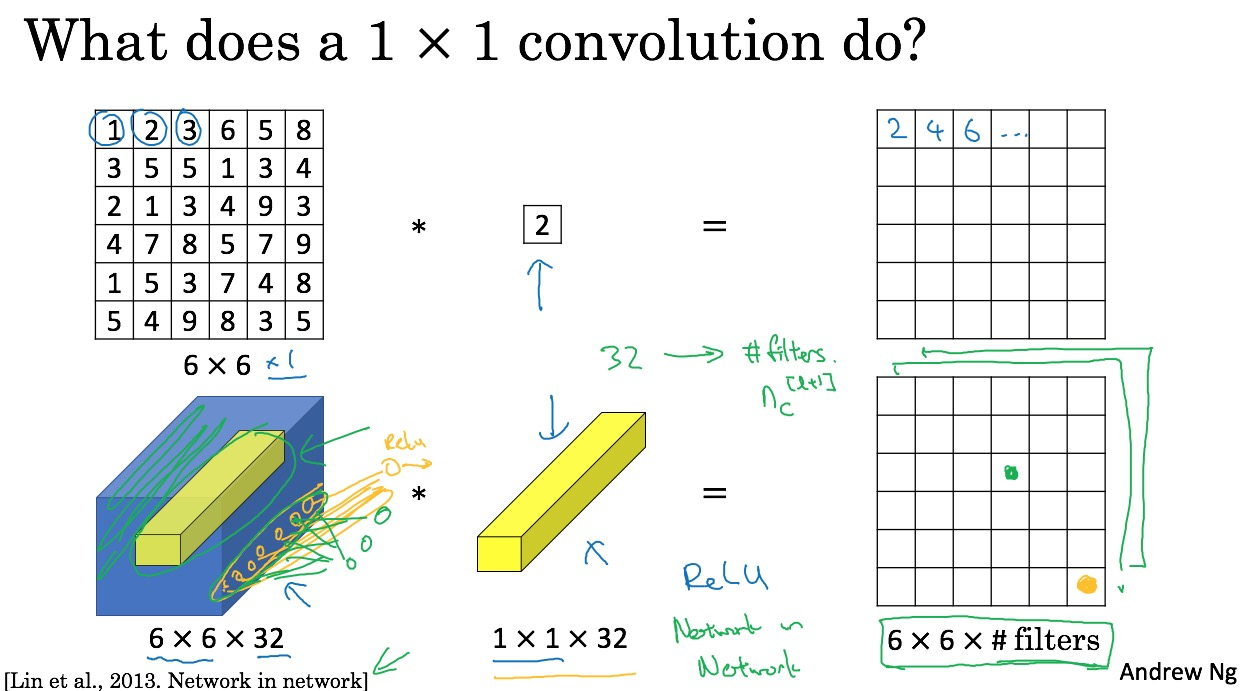
\includegraphics[width=40em]{figures/network-in-network}
    \caption{1 $\times$ 1 convolution (Network in Network)}
    \label{fig:network-in-network}
\end{figure}

Pooling layers can be used to shrink the height and width of a volume, while 1 $\times$
1 convolutions can be used to shink the channels to save on computation.

Just like Figure~\ref{fig:using-1-by-1-conv} shows, if you want to shrink the $28 \times 28 \times
192$ volume to $28 \times 28 \times 32$, you can use 32 $1 \times 1 \times 192$ filters to do 1
$\times$ 1 convolution with it, and you will get a $28 \times 28 \times 32$ output. If you keep the
number of channels at 192, that's fine, and the effect of a 1 $\times$ 1 convolution is it just
adds some nonlinearity, which allows you to learn more complex function of your network.

\begin{figure}[htb]
    \centering
    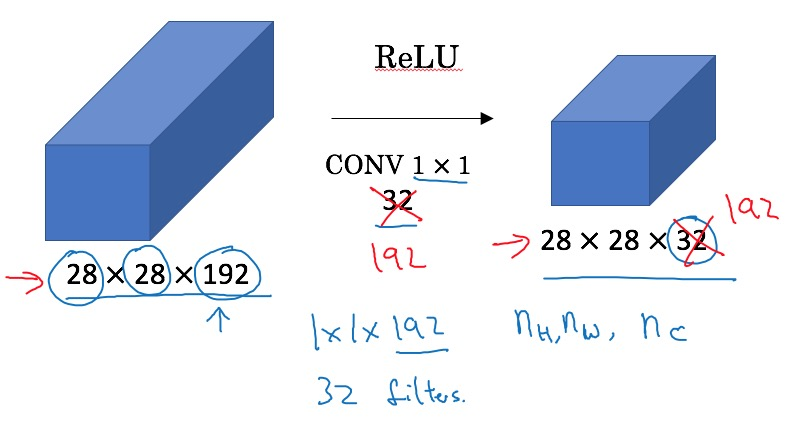
\includegraphics[width=40em]{figures/using-1-by-1-conv}
    \caption{Using 1 $\times$ 1 convolution to shrink the channels of a volume}
    \label{fig:using-1-by-1-conv}
\end{figure}

\subsubsection{Inception Network Motivation}
When designing a layer for a CONV layer, you might have to pick do you want $1 \times 3$ filter,
or $3 \times 3$, or $5 \times 5$. Or do you want to pooling layer? What inception network does is
it says, instead of choosing what filter size you want in a CONV layer or even do you want a
convolutional layer or pooling layer, let's do them all, see Figure~\ref{fig:inception-motivation}.

\begin{figure}[htb]
    \centering
    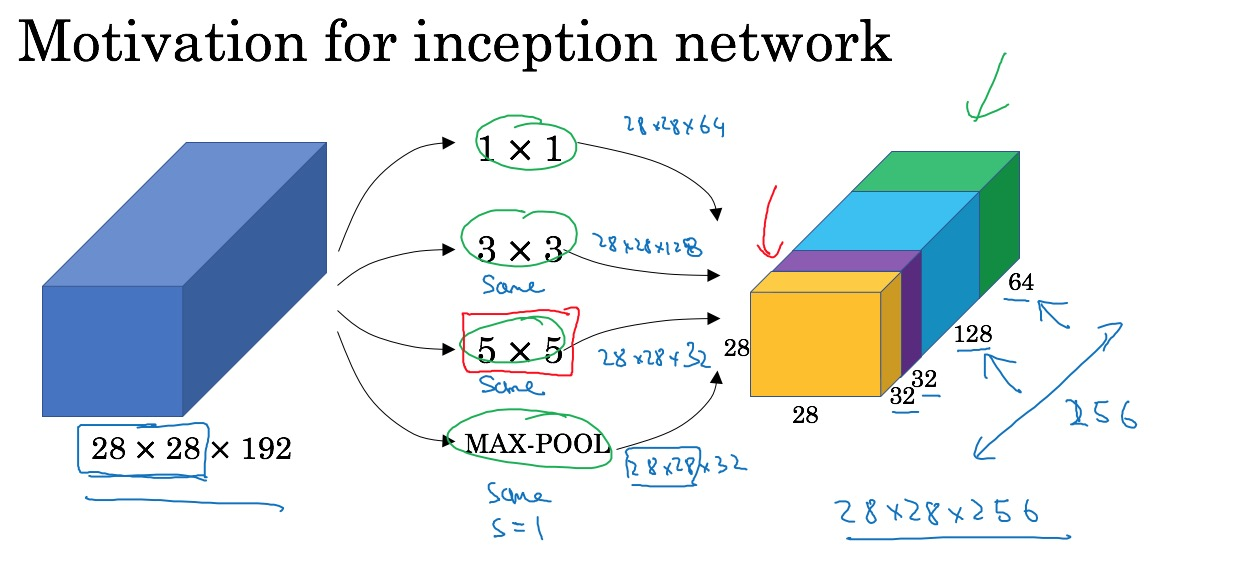
\includegraphics[width=40em]{figures/inception-motivation}
    \caption{The motivation for Inception Network}
    \label{fig:inception-motivation}
\end{figure}

\paragraph{The problem of computational cost}
Like Figure~\ref{fig:using-1-by-1-conv-to-save-computation}, with the help of ``bottleneck layer'',
you can save on computation by using 1 $\times$ 1 convolution.

\begin{figure}[htb]
    \centering
    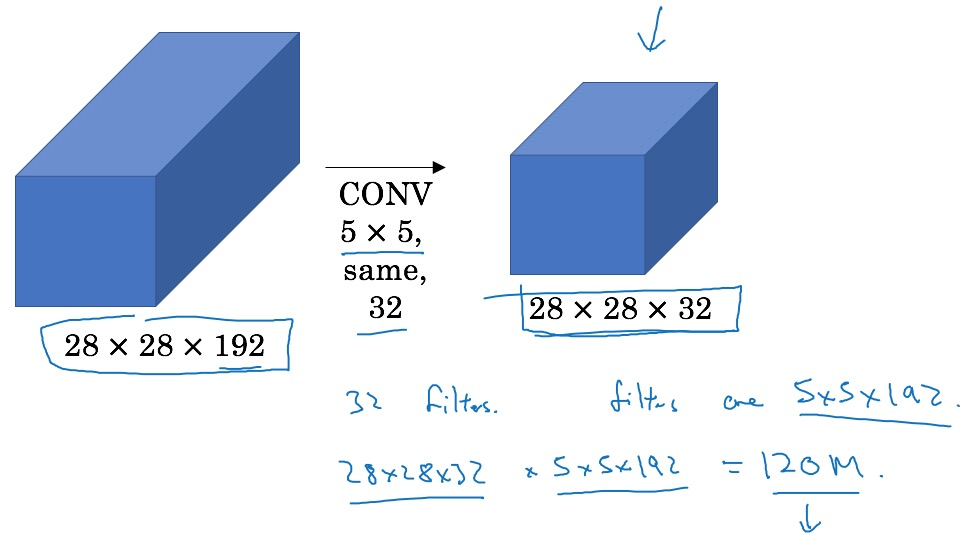
\includegraphics[width=30em]{figures/problem-of-computation-cost}
    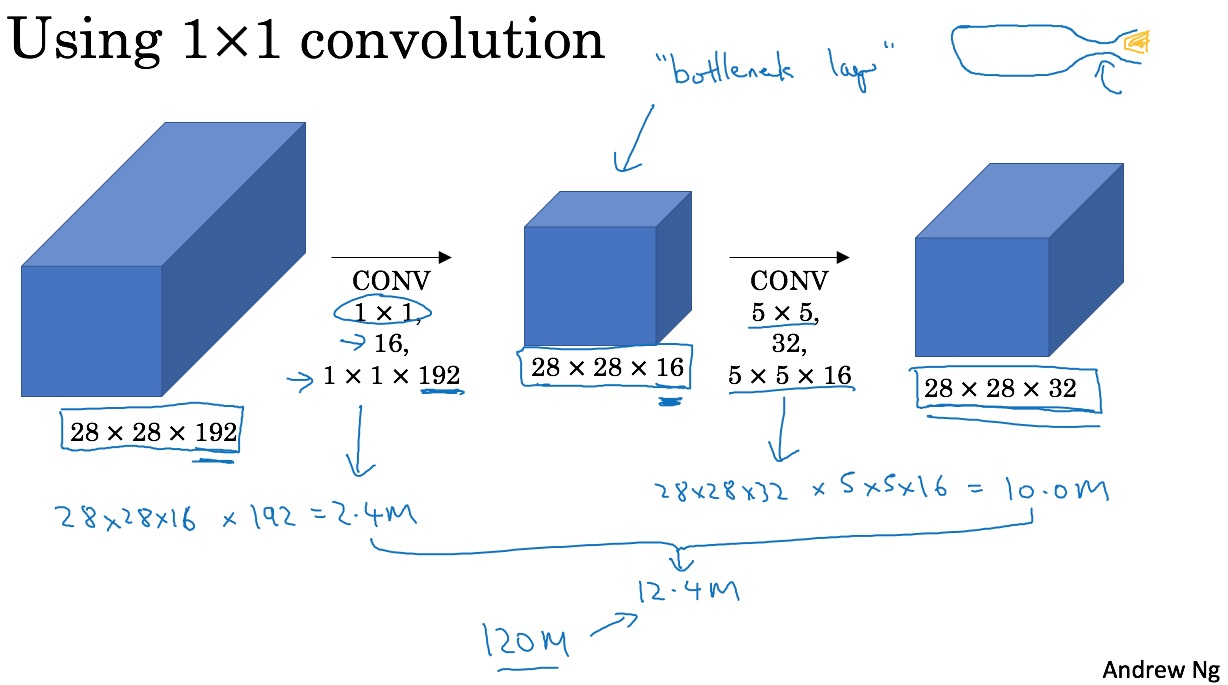
\includegraphics[width=40em]{figures/using-1-by-1-conv-to-save-computation}
    \caption{Using 1 $\times$ 1 convolution to save on computation.}
    \label{fig:using-1-by-1-conv-to-save-computation}
\end{figure}

\subsubsection{Inception Network}
Figure~\ref{fig:inception-module-and-inception-network} shows the Inception module and Inception
Network.

\begin{figure}[htb]
    \centering
    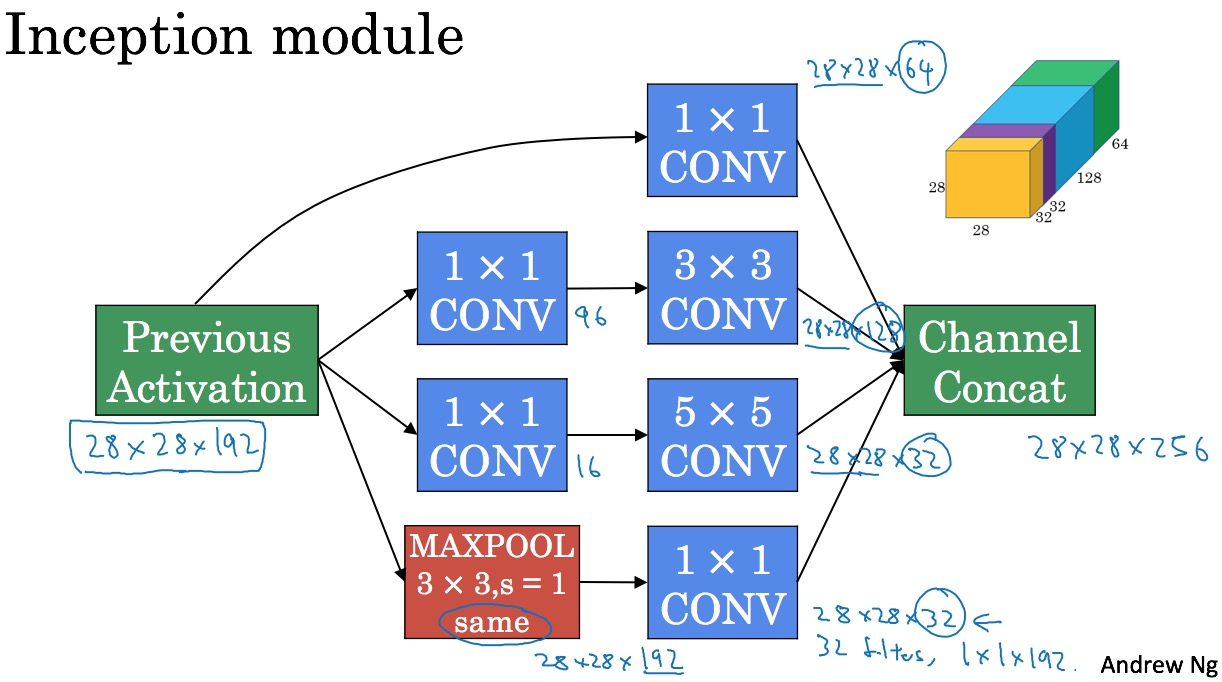
\includegraphics[width=25em]{figures/inception-module}
    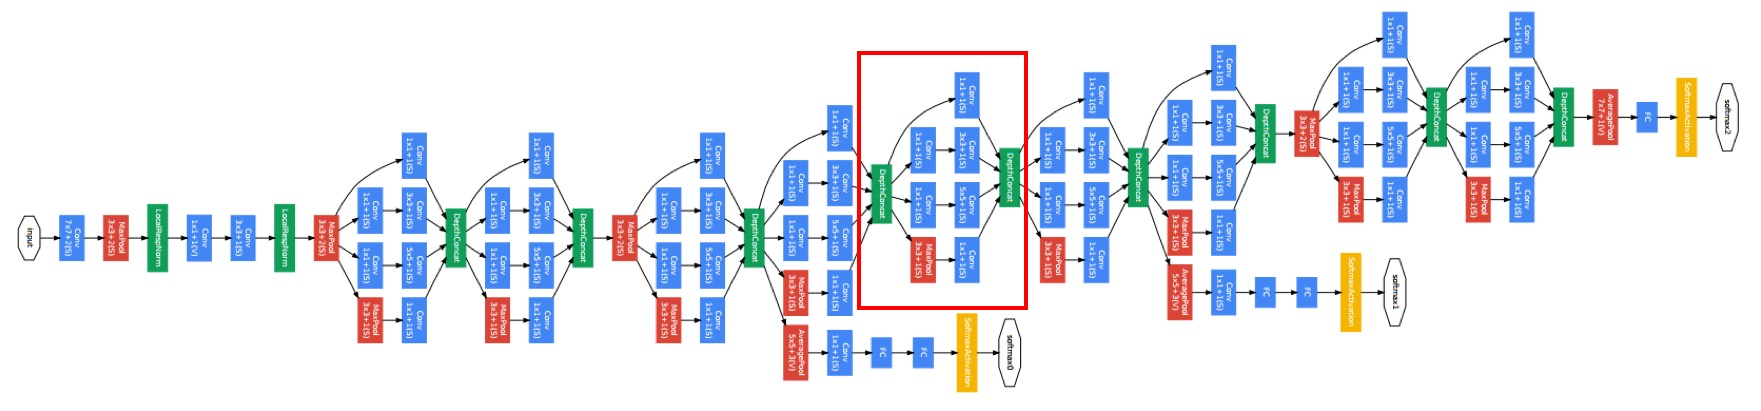
\includegraphics[width=40em]{figures/inception-network}
    \caption{Inception module and Inception Network}
    \label{fig:inception-module-and-inception-network}
\end{figure}

\subsubsection{Using Open-Source Implementation}
It turns out that a lot of effective neural networks are difficult or finicky to replicate because
a lot of details about tuning the hyperparameters such as learning rate and other things that make
some difference to the performance. Fortunately, a lot of deep learning researchers routinely open
source their work on the internet such as on GitHub.

If you're developing a computer vision application, a very common workflow would be to pick an
architecture that you'd like, and look for an open-source implementation and download it from
GitHub to start building from there. One of the advantages of doing so also is that sometimes these
networks take a long time to train and someone else might have used multiple GPUs in a very largely
dataset to pre-trained some of these networks. And that allows you to do transfer learning using
these networks.

\subsubsection{Transfer Learning}
If you're building a computer vision application, rather training the weights from scratch, from
random initialization, you often make much faster progress if you download weights that someone
else has already trained on a network architecture. And use that as pre-training and transfer that
to a new task that you might be interested in.

The computer vision community has been pretty good at hosting lots of datasets on the Internet. So
if you hear of things like ImageNet or MS COCO types of datasets, there are the names of different
datasets that people have posted online. And a lot of different researchers have trained their
algorithms on.

Sometimes this training takes several weeks, and might take many many GPUs. And the fact that
someone else has done this and gone through the painful high performance search process means that
you can often download open source weights that took someone else many weeks, or months to figure
out. And use that as a very good initialization for your own neural network. And use transfer
learning to sort of transfer knowledge from some of these very large public datasets to your own
problem.

Let's start an example, let's say you're building a cat detector to recognize your own pet cats
Tigger and Misty. So you have a classification problem with three classes, is this picture Tigger,
or is it Misty, or is it neither?

Now, you probably don't have a lot of pictures of Tigger and Misty, so your training set will be
small. You can go online and download some open source implementation of a neural network. And
download not just the code, but also the weights. And there are a lot of networks you can download
that have been trained on. For example, the ImageNet dataset, which has 1,000 different classes.
What you can do is then get rid of the softmax layer, and create your own softmax unit that outputs
Tigger, or Misty, or neither.

\begin{figure}[htb]
    \centering
    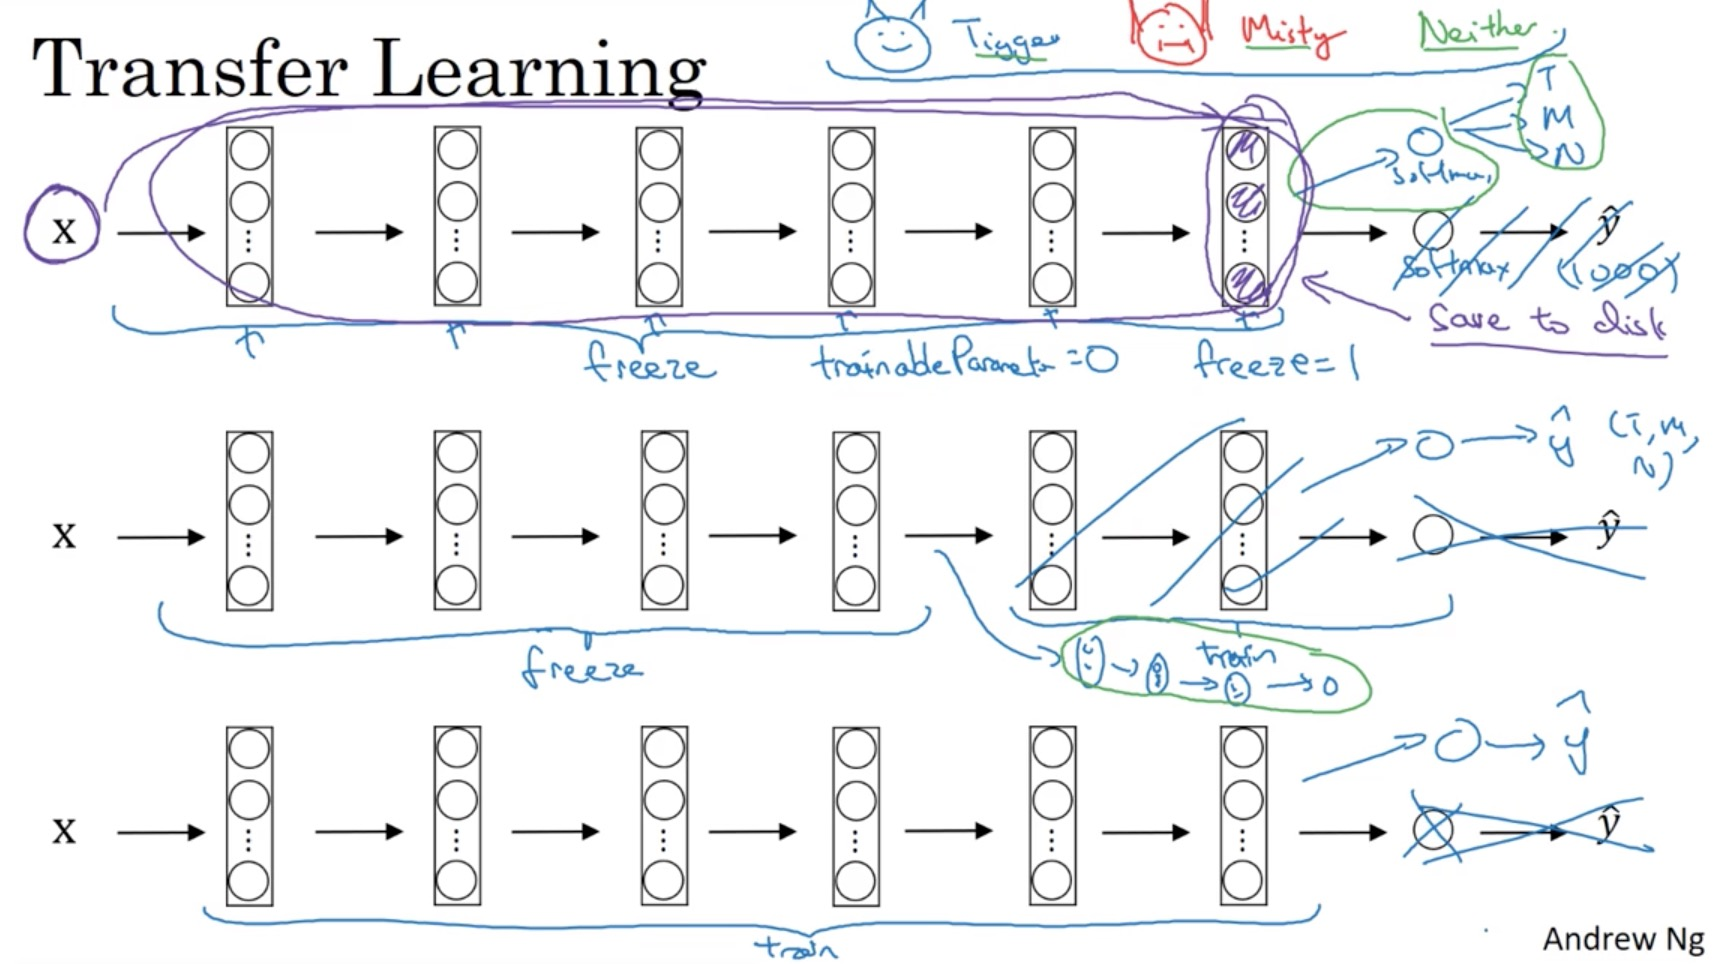
\includegraphics[width=40em]{figures/transfer-learning}
    \caption{Different ways of transfer learning.}
    \label{fig:transfer-learning}
\end{figure}

And in terms of the network, you can freeze the parameters in all the layers before softmax layer
and just train the parameters associated with softmax layer. By using someone else's pre-trained
weights, you're likely to get pretty good performance on this, even with a small dataset.

One other near trick that amy help for some permutations is that, because all of the earlier layers
are frozen, there is some fixed function that doesn't change, because you're not changing it,
you're not training it. That takes as input image $X$ and maps it to some sort of activations in
that layer. So one other trick that could speed up training is if we just pre-compute that layer,
the features or really activations from that layer, and just save them to disk. And what you're
doing is you're using this fixed function, in this part of the neural network, to take as input any
image $X$, and compute some feature vector for it. And then you're training a shallow softmax model
from this feature vector to make a prediction. And so one step that could help your computation is
you just pre-compute that layer's activation for all the examples in your training set, and save
them to disk. And then just train a softmax classifier on top of that. All right, so the advantages
of save to disk or the pre-compute method of save to disk method is that you don't need to recompute
those activations every time you take an epoch, or take a pass through your training set.

If you have a larger labeled dataset, so maybe you just have a ton of pictures of Tigger, Misty,
and as well as, I guess, pictures of neither of them. One thing you could do is then freeze fewer
layers, then train these left layers. And there are a couple of ways to do this, you could take the
last few layers' weights, and just use that as initilization and do gradient descent from there. Or
you could also blow away these last few layers, and just use your own new hidden units, and then
your own final softmax output. So either of these methods could be worth trying.

But maybe one pattern is, if you have more data, the number of layers you freeze could be smaller.
And then the number of layers you train on top could be greater.

\subsubsection{Data Augmentation}
Most computer vision tasks could use more data and so data augmentation is one of the techniques
that is often used to improve the performance of computer vision systems. Computer vision is a
pretty complicated task, and we say we just can't get enough data in this domain.

\begin{itemize}
    \item Common augmentation methods
    \begin{itemize}
        \item Mirroring
        \item Randon Cropping
        \item Rotation
        \item Shearing
        \item Local warping
        \item \ldots
    \end{itemize}
    \item Color shifting (e.g. PCA color augmentation)
\end{itemize}

If your dataset is very large, you can implement distortions (rotation, shearing, \ldots) during
training.

\subsubsection{State of Computer Vision}
If you have lots of data, you can use simpler algorithms, less hand-engineering; while if you have
little data, you need more hand-engineering.

When Andrew Ng looks at machine learning applications, he thinks usually the learning algorithm has
two sources of knowledge. One source knowledge is labeled data, the other is hand-engineering
features/network architectures/other components.

Tips for doing well on benchmarks/winning competitions:
\begin{itemize}
    \item Ensembling
    \begin{itemize}
        \item Train several networks independently and average their outputs
    \end{itemize}
    \item Multi-crop at test time
    \begin{itemize}
        \item Run classifier on multiple versions of test images and average results.
    \end{itemize}
\end{itemize}

Use open source code:
\begin{itemize}
    \item Use architectures of networks published in the literature
    \item Use open source implementations if possible
    \item Use pretrained models and fine-tune on your dataset
\end{itemize}
































\end{document}
